\externaldocument{../appendix/chapter_app}
\externaldocument{../4/chapter_algorithm}
\externaldocument{../3/chapter_modeling}
\startchapter{Proof of Concept}
\label{chapter:Exp}
In this section, I present two experiments I ran as a proof of concept of the communication analysis of two traces.

These experiments aimed to test the communication model and the communication analysis approach. They also verify the design of the some algorithms, for their correctness. I used the implemented features on Atlantis to conduct the experiments.

Among these two experiments, the first one was provided directly by our research partner DRDC with their initial requirement, while the second one was designed by me. In both experiments, DRDC conducted the programs execution and captured the traces on their environment while I performed the analysis locally with Atlantis on my desktop with the captured traces and corresponding .dll.

All test programs in these two experiments were written in C++ and the source code can be found in Appendix \ref{expcode}. Results are provided for each experiment. 

The experiments are restricted by the traces that can
be captured.  The current in-house tracer of DRDC is only able to capture the function information for named pipe function calls. So both of the conducted experiments used the named pipe communication method. 

I will describe the design of the experiments first. And then, I present the result of them with discussion of each one.

\section{Experiment 1}
\subsection{Experiment Design}
In the first experiment, two programs communicated with each other through a synchronous named pipe channel. One of the programs acted as the named pipe server while the other as the client. Figure \ref{exp1} is the sequence diagram of the interaction between the server and client. This sequence diagram only exemplify a possible sequence of the events. The actual events sequence can vary depending on the run-time environment. 


\begin{figure}[H]
\centerline{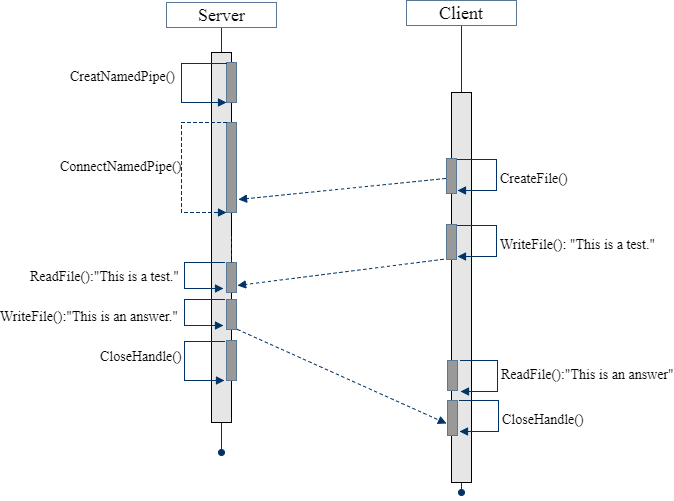
\includegraphics[scale=0.7]{Figures/exp1}}
 \caption{Sequence Diagram of Experiment 1}
\label{exp1}
\end{figure}

Two traces were captured while these two programs were running and interacting. The two captured traces, ``Sever.trace" and ``Client.trace" were analyzed as dual\_trace in this experiment. I used the implemented features in Atlantis to analyze this dual\_trace. I ran the ``Stream identification" and ``Communication identification" operations for this dual\_trace with the function descriptor as Table \ref{fdescexp1}. 

\begin{table}[H]
  \centering
  \caption{Function Descriptor of Named Pipe for Experiment 2}
  \label{fdescexp1}
  \begin{tabular}{|l|l|l|l|l|l|l|l|}
\hline
             \multirow{2}{*}{{\textbf{Name}}} & \multirow{2}{*}{{\textbf{Type}}} & \multicolumn{3}{c|}{\textbf{Input Parameters Description}} & \multicolumn{3}{c|}{\textbf{Output Parameters Description}} \\
              \cline{3-8} 
             & & \textbf{Name}& \textbf{Register} & \textbf{Addr/Val} & \textbf{Name}& \textbf{Register} &  \textbf{Addr/Val}  \\
             \hline
      CreateNamedPipeA
       &open & FileName & RCX  & Addr &  Handle & RAX & Val\\
      \hline         
      CreateFileA
       &open & FileName & RCX & Addr&  Handle & RAX & Val\\ 
      \hline              
      \multirow{2}{*}{WriteFile}
       &\multirow{2}{*}{send} &  Handle & RCX & Val & Length& R9 &Val\\
        \cline{3-8} 
       & & SendBuf & RDX & Addr & RetVal& RAX & Val\\
      \hline            
      \multirow{2}{*}{ReadFile}
       &\multirow{2}{*}{receive} &  Handle & RCX & Val& Length &R9 & Val\\
        \cline{3-8} 
       & & RecvBuf & RDX  & Addr & RetVal& RAX & Val\\
      \hline            
      CloseHandle &
       close &  Handle & RCX & Val & RetVal& RAX & Val\\
      \hline            
      DisconnectNamedPipe &
      close &  Handle & RCX & Val & RetVal& RAX & Val\\
      \hline               
  \end{tabular}
\end{table}



\subsection{Dual\_trace Analysis Result and Discussion}
$Client.trace$ has instruction lines. Four function call events were reconstructed from this trace as listed in Table \ref{funcclientexp1}.

\begin{table}[H]
  \centering
  \tiny
  \caption{The sequence of function call events of $Client.trace$}
  \label{funcclientexp1}
  \begin{tabular}{|l|p{16cm}|}
  \hline
\textbf{Line} & \multicolumn{1}{>{\centering\arraybackslash}m{16cm}|}{\textbf{Event}}\\
  \hline
  375744 & $funN:CreateFileA,  type:open, inparams:\lbrace Handle:F8, FileName:``\dot \backslash pipe \backslash mynamepipe" \rbrace, outparams:\lbrace RetVal:0 \rbrace$\\
 \hline
  385178 & $funN:WriteFile, type:send, inparams:\lbrace Handle:F8, SendBuf:``This\: is\: a\: test."\rbrace, outparams: \lbrace Length:15 \rbrace$\\
\hline
 391590&$funN:ReadFile, type:receive, inparams: \lbrace Handle:F8 \rbrace, outparams: \lbrace RecvBuf:``This\: is\: an\: answer", Length:17, RetVal:0 \rbrace$\\
\hline
 402442&$funN:CloseHandle, type:close, inparams: \lbrace Handle:F8 \rbrace, outparams: \lbrace RetVal:0 \rbrace$\\
\hline               
  \end{tabular}
\end{table}

All the values of the handle parameter of these four event are $F8$. So that a stream identified by the handle $F8$ was extracted, which consists of all these four function call events. 

$Server.trace$ has instruction lines. Five function call events were reconstructed from this trace as listed in Table \ref{funcserverexp1}.

\begin{table}[H]
  \centering
  \tiny
  \caption{The sequence of function call events of $Server.trace$}
  \label{funcserverexp1}
  \begin{tabular}{|l|p{16cm}|}
  \hline
\textbf{Line} & \multicolumn{1}{>{\centering\arraybackslash}m{16cm}|}{\textbf{Event}}\\
  \hline
  387947 & $funN:CreateNamedPipeA,  type:open, inparams:\lbrace Handle:F4, FileName:``\dot \backslash pipe \backslash mynamepipe" \rbrace, outparams:\lbrace RetVal:0 \rbrace$\\
 \hline
  431677&$funN:ReadFile, type:receive, inparams: \lbrace Handle:F4 \rbrace, outparams: \lbrace RecvBuf:``This\: is\: a\: test", Length:15, RetVal:0 \rbrace$\\
\hline
  436462 & $funN:WriteFile, type:send, inparams:\lbrace Handle:F4, SendBuf:``This\: is\: an\: answer."\rbrace, outparams: \lbrace Length:17 \rbrace$\\
\hline
 442158&$funN:DisconnectNamedPipe, type:close, inparams: \lbrace Handle:F4 \rbrace, outparams: \lbrace RetVal:0 \rbrace$\\
\hline   
 442224&$funN:CloseHandle, type:close, inparams: \lbrace Handle:F4 \rbrace, outparams: \lbrace RetVal:0 \rbrace$\\
\hline               
  \end{tabular}
\end{table}

All the values of the handle parameter of these four event are $F4$. So that a stream identified by the handle $F8$ was extracted, which consists of all these five function call events. 

The extracted streams are listed in the left table in the communication view as shown in Figure \ref{result1}.

In Table \ref{funcclientexp1}, the value of the FileName parameter of the channel open function call is $``\dot \backslash pipe \backslash mynamepipe"$. In Table \ref{funcserverexp1}, the value of the FileName parameter of the channel open function call is also $``\dot \backslash pipe \backslash mynamepipe"$. According to Algorithm \ref{streammatch}, the file name of a named pipe is treated as the channel identifier and used to match the communication. So that the stream in $Client.trace$ is matched to the stream in $Server.trace$.

There is only one send event and one receive event in both streams, the data verification of these two matched stream is trivial. The concatenation of the sent packets in the stream of $Client.trace$ and the concatenation of the received packets in the stream of $Server.trace$ are all $``This\: is\: a\: test."$. The concatenation of the sent packets in the stream of $Server.trace$ and the concatenation of the received packets in the stream of $Client.trace$ are all $``This\: is\: an\: answer."$. So these two match stream satisfy the content preservation of a communication. Therefore they are eventually output as a communication by the ``Communication Identification" operation as shown in the right table in Figure \ref{result1}.

In this experiment, ``Stream Extraction" operation is capable of properly extract the streams from both $Server.trace$ and $Client.trace$ while ``Communication Identification" operation is capable to identify the communication between the two traces.


\begin{figure}[H]
\centerline{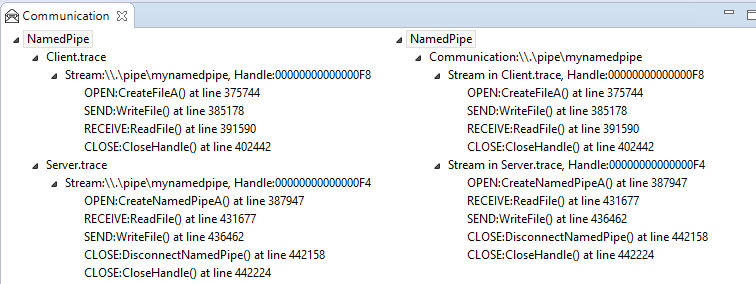
\includegraphics[scale=0.65]{Figures/result1}}
 \caption{Analysis Result of Dual\_trace in Experiment 1}
\label{result1}
\end{figure}


\section{Experiment 2}
\subsection{Experiment Design}
In the second experiment, a program was running as the named pipe server. In this server program, four named pipes were created and can be connected by up to four client at a time. Two other programs as the named pipe clients connected to this server. Those two clients (client 1 and client 2) used the identical program but run in sequence. Figure \ref{exp2} is the sequence diagram of the interaction among the server and clients. This sequence diagram only exemplify a possible sequence of the events. The actual events sequence can vary depending on the run-time environment. 


Three traces were captured at the time when these three programs were running and interacting. They are ``Server.trace" for the server program, ``Client1.trace" for the Client1 program and ``Client2.trace" for the Client2 program. These three traces are analyzed as two dual\_traces, one consist of ``Server.trace" and ``Client1.trace" while the other consist of ``Server.trace" and ``Client2.trace". I performed the ``Stream Extraction" and ``Communication Identification" operations for these two dual\_traces with the function descriptor as Table \ref{fdescexp2}.



\begin{table}[H]
  \centering
  \caption{Function Descriptor of Named Pipe for Experiment 2}
  \label{fdescexp2}
\begin{tabular}{|l|l|l|l|l|l|l|l|}
\hline
             \multirow{2}{*}{{\textbf{Name}}} & \multirow{2}{*}{{\textbf{Type}}} & \multicolumn{3}{c|}{\textbf{Input Parameters Description}} & \multicolumn{3}{c|}{\textbf{Output Parameters Description}} \\
              \cline{3-8} 
             & & \textbf{Name}& \textbf{Register} & \textbf{Addr/Val} & \textbf{Name}& \textbf{Register} &  \textbf{Addr/Val}  \\
             \hline
      CreateNamedPipe
       &open & FileName & RCX  & Addr &  Handle & RAX & Val\\
      \hline         
      CreateFile
       &open & FileName & RCX & Addr&  Handle & RAX & Val\\ 
      \hline              
      \multirow{2}{*}{WriteFile}
       &\multirow{2}{*}{send} &  Handle & RCX & Val & Length & R9 & Val\\
        \cline{3-8} 
       & & SendBuf & RDX & Addr & RetVal& RAX & Val\\
      \hline            
      \multirow{2}{*}{ReadFile}
       &\multirow{2}{*}{receive} &  Handle & RCX & Val& Length & R9 & Val\\
        \cline{3-8} 
       & & RecvBuf & RDX  & Addr & RetVal& RAX & Val\\
      \hline    
           \multirow{2}{*}{GetOverlappedResult} &
       \multirow{2}{*}{receive} &  \multirow{2}{*}{Handle} & \multirow{2}{*}{RCX} & \multirow{2}{*}{Val} &OverlapStruct &RDX & Addr\\
               \cline{6-8} 
       & &  &   &  & RetVal& RAX & Val\\
      \hline     
      CloseHandle &
       close &  Handle & RCX & Val & RetVal& RAX & Val\\
      \hline            
      DisconnectNamedPipe &
      close &  Handle & RCX & Val & RetVal& RAX & Val\\
      \hline               
  \end{tabular}  
\end{table} 

\begin{figure}[H]
\centerline{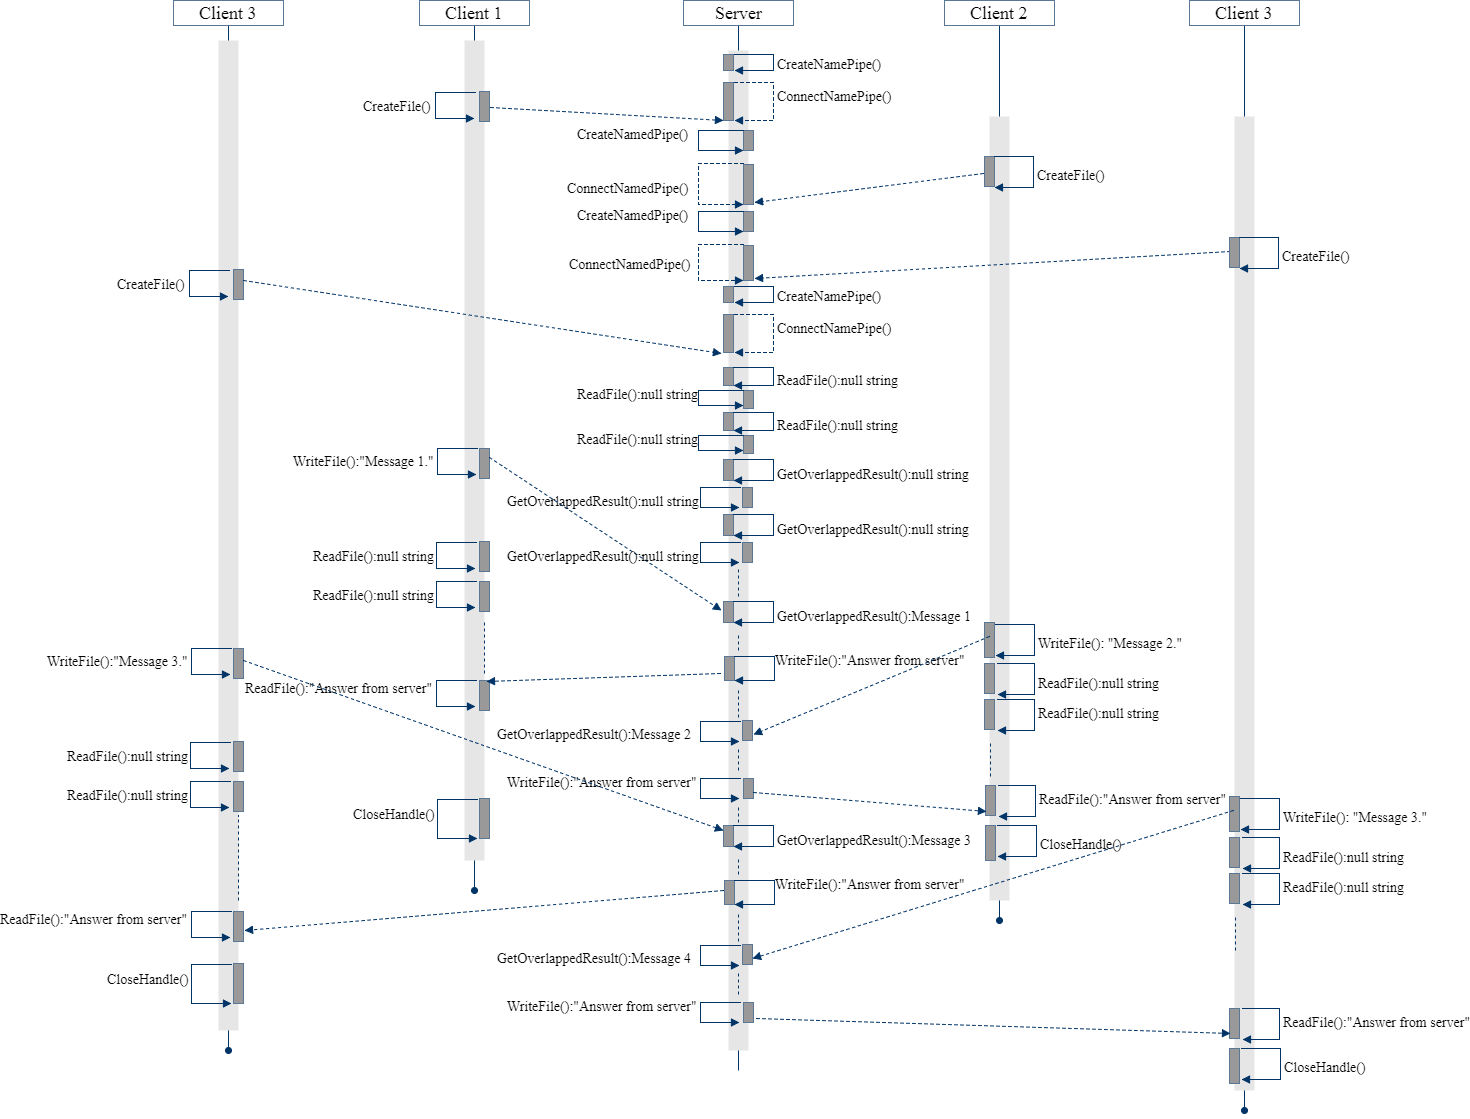
\includegraphics[scale=0.6]{Figures/exp2}}
 \caption{Sequence Diagram of Experiment 2}
\label{exp2}
\end{figure}


\subsection{Dual\_trace Analysis Result  and Discussion}
\subsubsection{Dual\_trace: $Server.trace$ and $Client1.trace$}
$Client1.trace$ has instruction lines. Four function call events were reconstructed from this trace as listed in Table \ref{funcclient1exp2}.

\begin{table}[H]
  \centering
  \tiny
  \caption{The sequence of function call events of $Client1.trace$}
  \label{funcclient1exp2}
  \begin{tabular}{|l|p{16cm}|}
  \hline
\textbf{Line} & \multicolumn{1}{>{\centering\arraybackslash}m{16cm}|}{\textbf{Event}}\\
  \hline
  1723886 & $funN:CreateFileA,  type:open, inparams:\lbrace Handle:114, FileName:``\dot \backslash pipe \backslash mynamepipe" \rbrace, outparams:\lbrace RetVal:0 \rbrace$\\
 \hline
  1734413 & $funN:WriteFile, type:send, inparams:\lbrace Handle:114, SendBuf:``Message\:1"\rbrace, outparams: \lbrace Length:15 \rbrace$\\
\hline
 1740825&$funN:ReadFile, type:receive, inparams: \lbrace Handle:114 \rbrace, outparams: \lbrace RecvBuf:``Default\: answer\: from \: server", Length:17, RetVal:0 \rbrace$\\
\hline
 1752640&$funN:CloseHandle, type:close, inparams: \lbrace Handle:114 \rbrace, outparams: \lbrace RetVal:0 \rbrace$\\
\hline               
  \end{tabular}
\end{table}

All the values of the handle parameter of these four event are $114$. So that a stream identified by the handle $114$ was extracted, which consists of all these four function call events. 

$Server.trace$ has instruction lines. Ten function call events were reconstructed from this trace as listed in Table \ref{funcserverexp1}.

\begin{table}[H]
  \centering
  \tiny
  \caption{The sequence of function call events of $Server.trace$}
  \label{funcserverexp1}
  \begin{tabular}{|l|p{16cm}|}
  \hline
\textbf{Line} & \multicolumn{1}{>{\centering\arraybackslash}m{16cm}|}{\textbf{Event}}\\
  \hline
  1732413 & $funN:CreateNamedPipeA,  type:open, inparams:\lbrace Handle:118, FileName:``\dot \backslash pipe \backslash mynamepipe" \rbrace, outparams:\lbrace RetVal:0 \rbrace$\\
 \hline
   1741477 & $funN:CreateNamedPipeA,  type:open, inparams:\lbrace Handle:120, FileName:``\dot \backslash pipe \backslash mynamepipe" \rbrace, outparams:\lbrace RetVal:0 \rbrace$\\
 \hline
   1749553 & $funN:CreateNamedPipeA,  type:open, inparams:\lbrace Handle:128, FileName:``\dot \backslash pipe \backslash mynamepipe" \rbrace, outparams:\lbrace RetVal:0 \rbrace$\\
 \hline
   1757626 & $funN:CreateNamedPipeA,  type:open, inparams:\lbrace Handle:130, FileName:``\dot \backslash pipe \backslash mynamepipe" \rbrace, outparams:\lbrace RetVal:0 \rbrace$\\
 \hline
  1765950&$funN:ReadFile, type:receive, inparams: \lbrace Handle:118 \rbrace, outparams: \lbrace RecvBuf:``Message\: 2", Length:15, RetVal:0 \rbrace$\\
\hline
  1770738 & $funN:WriteFile, type:send, inparams:\lbrace Handle:118, SendBuf:``Default\: answer\: from\: server"\rbrace, outparams: \lbrace Length:17 \rbrace$\\
\hline
  1771676&$funN:ReadFile, type:receive, inparams: \lbrace Handle:120 \rbrace, outparams: \lbrace RecvBuf:``Message\: 1", Length:15, RetVal:0 \rbrace$\\
\hline
  1775507 & $funN:WriteFile, type:send, inparams:\lbrace Handle:120, SendBuf:``Default\: answer\: from\: server"\rbrace, outparams: \lbrace Length:17 \rbrace$\\
\hline
 1777180&$funN:DisconnectNamedPipe, type:close, inparams: \lbrace Handle:118 \rbrace, outparams: \lbrace RetVal:0 \rbrace$\\
\hline   
 1778658&$funN:DisconnectNamedPipe, type:close, inparams: \lbrace Handle:120 \rbrace, outparams: \lbrace RetVal:0 \rbrace$\\
\hline               
  \end{tabular}
\end{table}

There are four handle values in this event sequence: $118$, $120$, $128$, $130$. So four streams are extracted with these four identifiers. Both stream $118$ and $120$ have four events while stream $128$ and $130$ only have one channel open event. 

The extracted streams are listed in the left table in the communication view as shown in Figure \ref{result21}.

In Table \ref{funcclient1exp2}, the value of the FileName parameter of the channel open function call is $``\dot \backslash pipe \backslash mynamepipe"$. In Table \ref{funcserverexp2}, the value of the FileName parameter of all channel open function calls are also $``\dot \backslash pipe \backslash mynamepipe"$. So that all streams of $Server.trace$ will be matched to the only one stream of $Client1.trace$ by the stream matching algorithm.

However, only the stream $120$ of $Server.trace$ and the stream of $Client1.trace$ can satisfy the content preservation of a communication. Therefore they are eventually output as a communication by the ``Communication Identification" operation as shown in the right table in Figure \ref{result21}. 


\begin{figure}[H]
\centerline{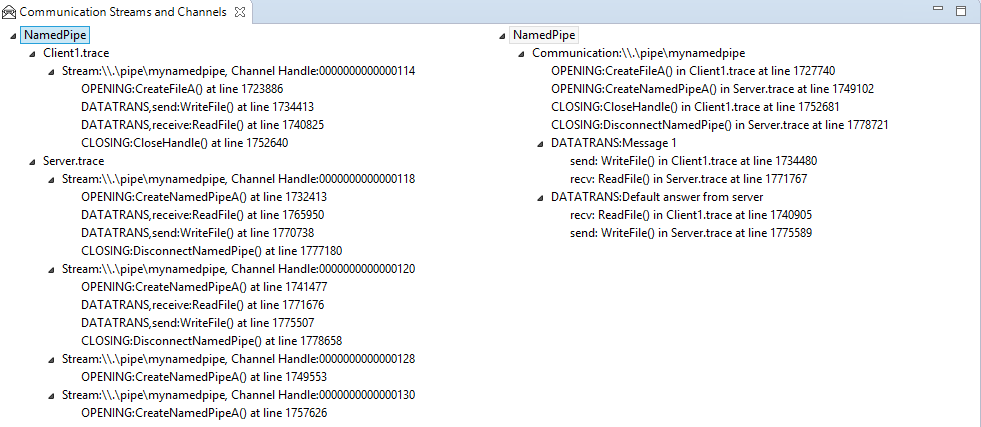
\includegraphics[scale=0.55]{Figures/result21}}
 \caption{Analysis Result of the Dual\_trace:``Server.trace" and ``Client1.trace" in Experiment 2}
\label{result21}
\end{figure}

\subsubsection{Dual\_trace: $Server.trace$ and $Client2.trace$}
$Client2.trace$ has instruction lines. Four function call events were reconstructed from this trace as listed in Table \ref{funcclient2exp2}.

\begin{table}[H]
  \centering
  \tiny
  \caption{The sequence of function call events of $Client1.trace$}
  \label{funcclient2exp2}
  \begin{tabular}{|l|p{16cm}|}
  \hline
\textbf{Line} & \multicolumn{1}{>{\centering\arraybackslash}m{16cm}|}{\textbf{Event}}\\
  \hline
  1723886 & $funN:CreateFileA,  type:open, inparams:\lbrace Handle:114, FileName:``\dot \backslash pipe \backslash mynamepipe" \rbrace, outparams:\lbrace RetVal:0 \rbrace$\\
 \hline
  1734413 & $funN:WriteFile, type:send, inparams:\lbrace Handle:114, SendBuf:``Message\:1"\rbrace, outparams: \lbrace Length:15 \rbrace$\\
\hline
 1740825&$funN:ReadFile, type:receive, inparams: \lbrace Handle:114 \rbrace, outparams: \lbrace RecvBuf:``Default\: answer\: from \: server", Length:17, RetVal:0 \rbrace$\\
\hline
 1752640&$funN:CloseHandle, type:close, inparams: \lbrace Handle:114 \rbrace, outparams: \lbrace RetVal:0 \rbrace$\\
\hline               
  \end{tabular}
\end{table}

All the values of the handle parameter of these four event are $114$. So that a stream identified by the handle $114$ was extracted, which consists of all these four function call events. 

Same as the last Dual\_trace, all streams of $Server.trace$ will be matched to the only one stream of $Client2.trace$ by the stream matching algorithm.

However, only the stream $118$ of $Server.trace$ and the stream of $Client2.trace$ can satisfy the content preservation of a communication. Therefore they are eventually output as a communication by the ``Communication Identification" operation as shown in the right table in Figure \ref{result22}. 

\begin{figure}[H]
\centerline{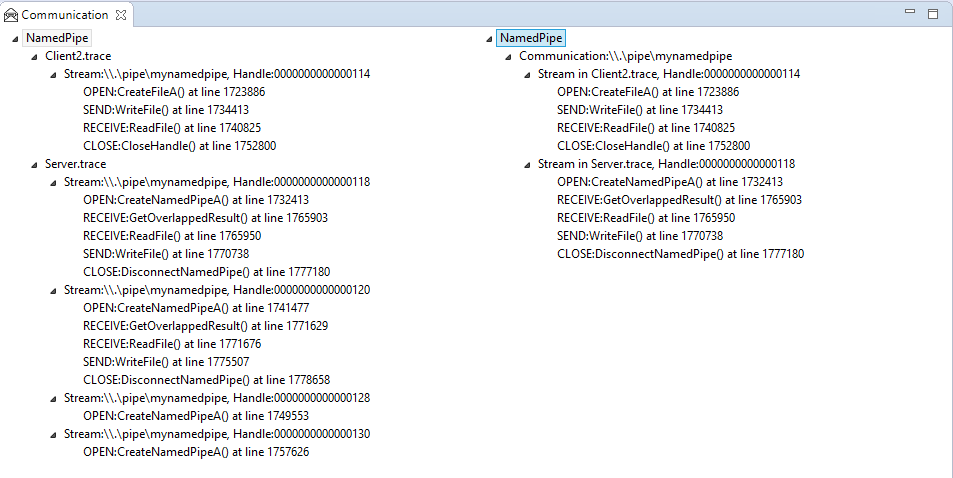
\includegraphics[scale=0.55]{Figures/result22}}
 \caption{Analysis Result of the Dual\_trace:``Server.trace" and ``Client2.trace" in Experiment 2}
\label{result22}
\end{figure}

\subsubsection{Discussion for Both Dual\_traces}
In this experiment, ``Stream Extraction" operation is capable of properly extract the streams from both $Server.trace$, $Client1.trace$ and $Client2.trace$ while ``Communication Identification" operation is capable to identify the communications between the two traces in the analysis of the both dual\_trace. 






   




